Este cap\'{i}tulo describe el proceso seguido para la generaci\'{o}n del modelo de detecci\'{o}n de anomal\'{i}as de manejo. Seg\'{u}n lo repasado en el cap\'{i}tulo anterior, en el presente trabajo, se propone un m\'{e}todo de detecci\'{o}n de anomal\'{i}as de conducci\'{o}n siguiendo un enfoque semi-supervisado; sin embargo, antes de profundizar en el m\'{e}todo propuesto se debe realizar un repaso del conjunto de datos con el que se cuenta en la investigaci\'{o}n.

\section{Conjunto de datos normales y an\'{o}malos}

En el Cap\'{i}tulo 3 se describi\'{o} el proceso de captura y preparaci\'{o}n del conjunto de datos, as\'{i} como tambi\'{e}n su divisi\'{o}n en conjunto de entrenamiento/desarrollo/prueba; sin embargo cabe aclarar que aquel cap\'{i}tulo s\'{o}lo se enfoc\'{o} en el  \textbf{conjunto de datos normales}, los cuales corresponden a aquellos datos que no cuentan con una etiqueta.%; por lo que es el conjunto que se usa para entrenar el modelo que se ajusta al comportamiento normal de manejo.

\vspace{5mm} %5mm vertical space

A pesar de contar con una gran cantidad de datos normales se debe recolectar datos que correspondan a anomal\'{i}as con el objetivo de poder validar el m\'{e}todo que se propone en este proyecto. Por lo que se debi\'{o} proceder a la captura de  \textbf{datos an\'{o}malos}, el cual est\'{a} conformado seg\'{u}n el Cuadro \ref{table:conjunto_anomalias}.

\begin{table}[]
\centering
\begin{tabular}{|l|l|l|}
\hline
Tipo de anomal\'{i}a & Nro anomal\'{i}as & Nro de datos \\ \hline
Frenos en seco    & 5  & 100  \\ \hline
Giros a la derecha e izquierda a alta velocidad & 5  & 450  \\ \hline
Giros en U a alta velocidad & 5 & 300 \\ \hline
\end{tabular}
\caption{Tabla del conjunto de anomal\'{i}as.}
\label{table:conjunto_anomalias}
\end{table}

\vspace{5mm} %5mm vertical space

Como se mencion\'{o} en el anterior p\'{a}rrafo el conjunto de anomal\'{i}as fue capturado para validar el m\'{e}todo propuesto, por lo que este conjunto ser\'{a} etiquetado como positivo (con la etiqueta 1) y el conjunto de datos normales ser\'{a} etiquetado como muestras negativas (con la etiqueta 0).

\subsection{Generaci\'{o}n de series temporales}

Para la generaci\'{o}n del modelo detector de anomal\'{i}as se opt\'{o} por algoritmos de aprendizaje autom\'{a}tico enfocados en series de tiempo, dado que los datos capturados por el dispositivo m\'{o}vil, dependen del tiempo en el que fueron capturados; por lo cual el primer paso a realizar es la generaci\'{o}n de peque\~{n}as fracciones de series temporales, esto permitir\'{a} que el modelo propuesto vaya m\'{a}s all\'{a} de una simple detecci\'{o}n de anomal\'{i}as puntuales y pueda detectar anomal\'{i}as contextuales o colectivas.

\vspace{5mm} %5mm vertical space

En el Cuadro \ref{table:series-de-tiempo} se presenta los resultados de diferentes tama\~{n}os de series de tiempo, observando estos resultados en primera instancia se descarta la serie de tiempo que cuenta con uno y dos pasos; debido a que no son lo suficientemente descriptivos. En cuanto a las series de tiempo restantes no es posible definir a\'{u}n cual es la cantidad correcta de pasos, por lo cual al igual que la cantidad de componentes principales, ser\'{a} un par\'{a}metro a optimizar en los diferentes experimentos que se realizar\'{a} en las siguientes secciones. Cabe recalcar que el dominio de \'{e}sta variable estar\'{a} entre 3 a 5 pasos y el de la cantidad de componentes principales estar\'{a} entre 3 y 4.

\begin{table}[]
\centering
\begin{center}
\begin{tabular}{cl|l|l|}
\cline{3-4}
\multicolumn{1}{l}{} &   & \multicolumn{2}{c|}{\textbf{Nro de componentes}} \\ \cline{3-4} 
\multicolumn{1}{l}{} &   & \multicolumn{1}{c|}{3} & \multicolumn{1}{c|}{4} \\ \hline
\multicolumn{1}{|c|}{\multirow{5}{*}{\rotatebox{90}{\textbf{Tama\~{n}os de series de tiempo}}}} & \multicolumn{1}{c|}{1} & \adj{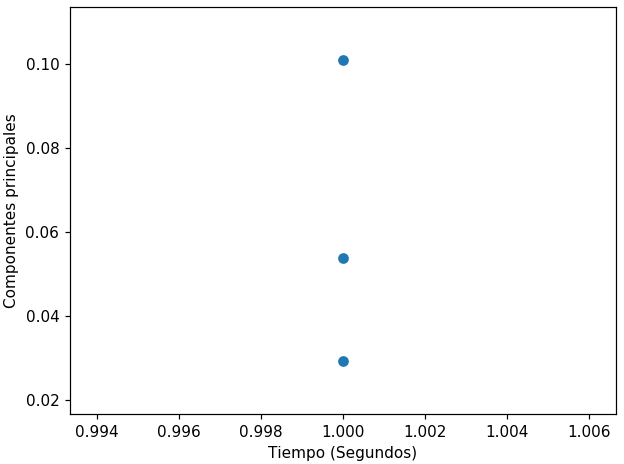
\includegraphics[width=1.85in]{imagenes/Cap4/pca3-1}} & \adj{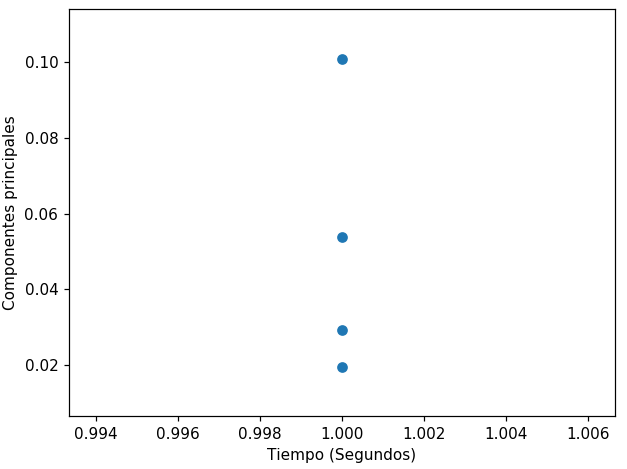
\includegraphics[width=1.85in]{imagenes/Cap4/pca4-1}}  \\ \cline{2-4} 
\multicolumn{1}{|c|}{}                                             & \multicolumn{1}{c|}{2} & \adj{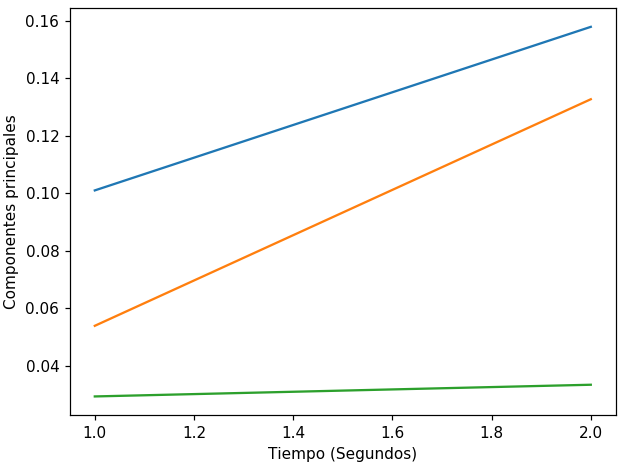
\includegraphics[width=1.85in]{imagenes/Cap4/pca3-2}}  & \adj{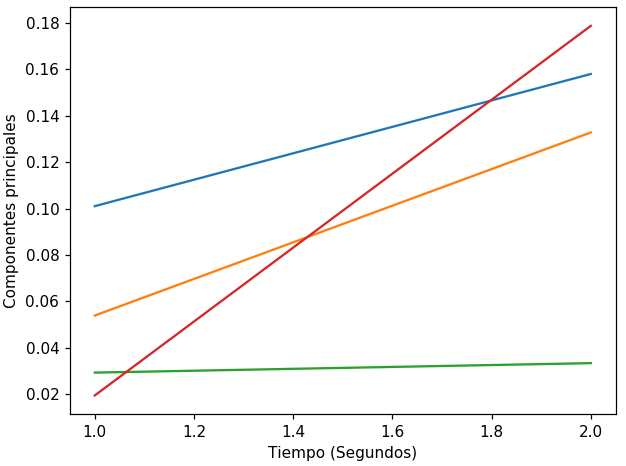
\includegraphics[width=1.85in]{imagenes/Cap4/pca4-2}} \\ \cline{2-4} 
\multicolumn{1}{|c|}{}                                             & 3 & \adj{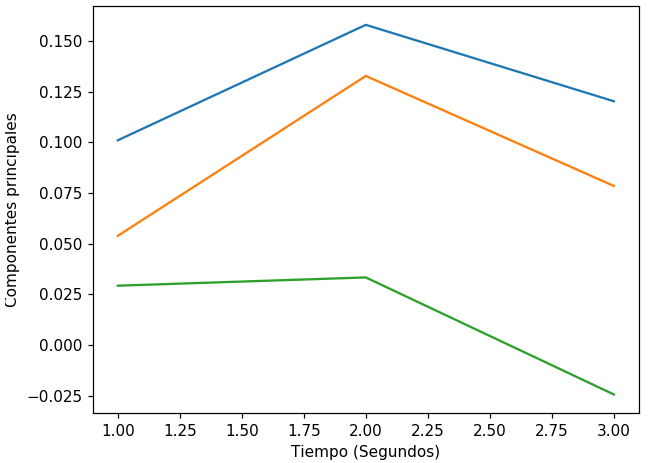
\includegraphics[width=1.85in]{imagenes/Cap4/pca3-3}} & \adj{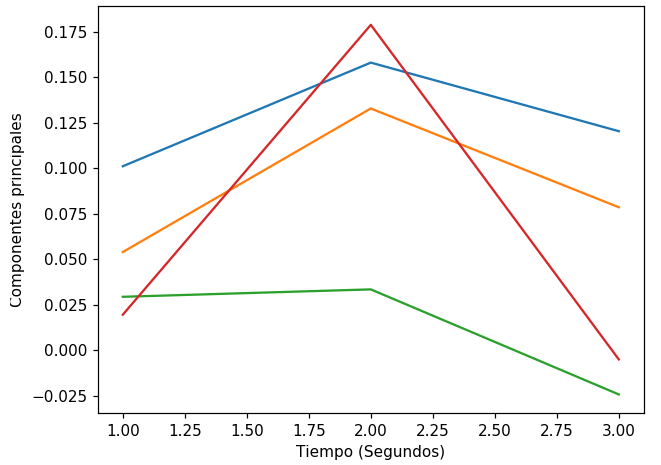
\includegraphics[width=1.85in]{imagenes/Cap4/pca4-3}} \\ \cline{2-4} 
\multicolumn{1}{|c|}{}                                             & 4 & \adj{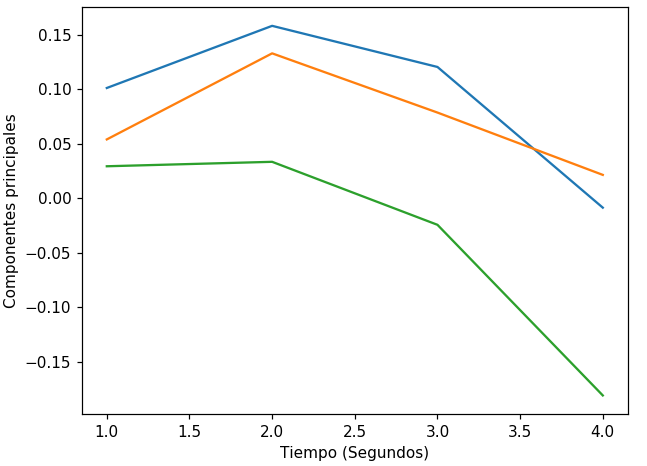
\includegraphics[width=1.85in]{imagenes/Cap4/pca3-4}} & \adj{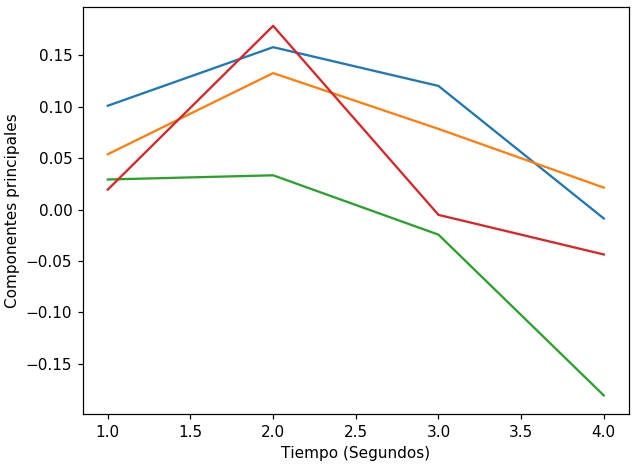
\includegraphics[width=1.85in]{imagenes/Cap4/pca4-4}} \\ \cline{2-4} 
\multicolumn{1}{|c|}{}                                             & 5 & \adj{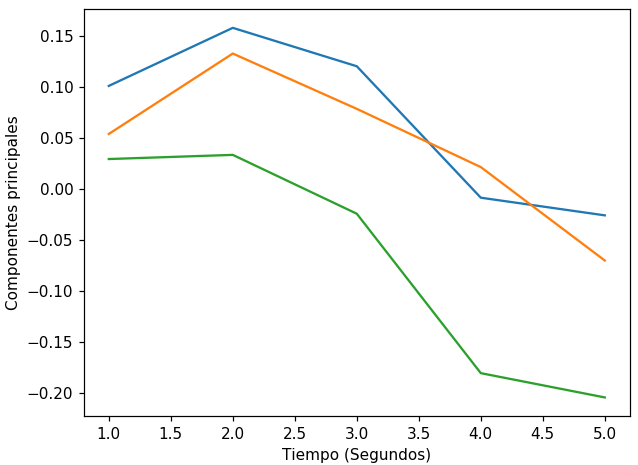
\includegraphics[width=1.85in]{imagenes/Cap4/pca3-5}} & \adj{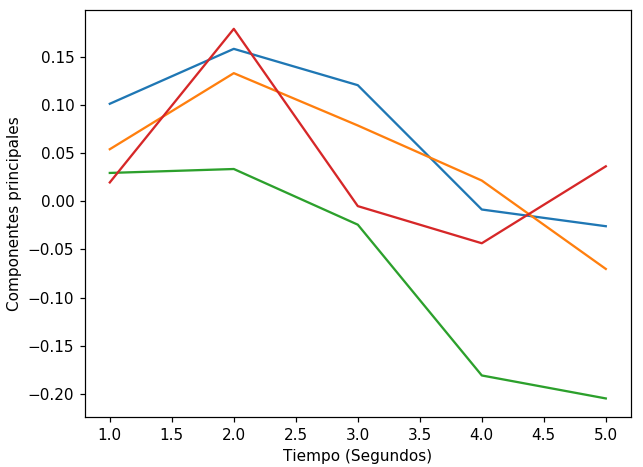
\includegraphics[width=1.85in]{imagenes/Cap4/pca4-5}} \\ \hline
\end{tabular}
\end{center}
\caption{Tabla con diferentes tama\~{n}os de series de tiempo para 3 y 4 componentes principales.}
  \label{table:series-de-tiempo}
\end{table}

\section{Modelo de detecci\'{o}n de anomal\'{i}as}

Como se mencion\'{o} previamente en la presente investigaci\'{o}n se propone un m\'{e}todo de detecci\'{o}n de anomal\'{i}as de conducci\'{o}n siguiendo un enfoque semi-supervisado, el cual consta de dos componentes: un \textbf{modelo ajustado al comportamiento normal} de manejo de un agente y un \textbf{m\'{e}todo de umbral para la detecci\'{o}n de valores at\'{i}picos}.

\vspace{5mm} %5mm vertical space

Para la presente investigaci\'{o}n se har\'{a} la comparaci\'{o}n entre 3 diferentes m\'{e}todos de detecci\'{o}n, y seg\'{u}n el rendimiento de cada uno se elegir\'{a} la mejor opci\'{o}n. En el Cuadro \ref{table:metodos_comparados} se presenta los tres diferentes m\'{e}todos que ser\'{a}n comparados y como se puede observar para todos los casos se usa un autoencoder como modelo del comportamiento normal, por lo que las siguientes secci\'{o}nes se enfocar\'{a}n en la descripci\'{o}n del entrenamiento del autoencoder, para posteriormente probar los 3 diferentes tipos de detecci\'{o}n de anomal\'{i}as.

\begin{table}[H]
\centering
\begin{tabular}{|l|p{100mm}|}
\hline
\textbf{M\'{e}todo} & \textbf{Descripci\'{o}n} \\ \hline
AE\_T & M\'{e}todo de detecci\'{o}n basado en autoencoders y umbralizaci\'{o}n (Thresholding) \\ \hline
AE\_IF & M\'{e}todo de detecci\'{o}n basado en autoencoders y la aplicaci\'{o}n de Isolation Forest sobre la codificaci\'{o}n obtenida por el autoencoder  \\ \hline
AE\_OC-SVM & M\'{e}todo de detecci\'{o}n basado en autoencoders y la aplicaci\'{o}n de One-Class SVM sobre la codificaci\'{o}n obtenida por el autoencoder \\ \hline
\end{tabular}
\caption{Tabla de los m\'{e}todos comparados.}
\label{table:metodos_comparados}
\end{table}

\subsection{Modelo del comportamiento normal}

Esta etapa es una de las partes m\'{a}s importantes de \'{e}ste trabajo debido a que el rendimiendo del modelo de detecci\'{o}n de anomal\'{i}as depende en gran parte de la precisi\'{o}n de esta etapa.

\subsubsection{Arquitectura del modelo}

Como se mencion\'{o} en la anterior secci\'{o}n en esta etapa se utilizar\'{a} un autoencoder como modelo ajustado al comportamiento normal de manejo. Por lo cual el autoencoder se entren\'{o} con el conjunto de datos normales, de manera que el modelo aprenda a generar s\'{o}lo las clases que se consideran normales y, con suerte, tendr\'{a} problemas para reconstruir anomal\'{i}as, debido a que estas muestras no fueron presentadas durante el entrenamiento.

\vspace{5mm} %5mm vertical space

Para ello se prob\'{o} con diferentes arquitecturas, primero la forma m\'{a}s simple que solo se basa el uso de capas densas, luego se hizo pruebas con redes convolucionales y por \'{u}ltimo con redes recurrentes haciendo uso espec\'{i}fico de capas LSTM. Por cada tipo de red se hizo la prueba con 6 diferentes tipos de combinaciones de entrada, como se indica en el Cuadro \ref{table:series-de-tiempo}, es decir, se prob\'{o} una diferente cantidad de pasos (entre 3 y 5) por cada cantidad de componentes principales (3 y 4). Por lo tanto se realizaron 18 diferentes experimentos, de los cuales por cada tipo de red sobresalio uno (usando la precisi\'{o}n de las redes como tipo de evaluaci\'{o}n para desarrollar las comparaciones).

\vspace{5mm} %5mm vertical space

En el Cuadro \ref{table:dense33} se presenta la mejor red de todas las Redes Densas que se probaron, esta red corresponde a la red que fue alimentada con 3 componentes principales en secuencias de 3 pasos. Esta red cuenta con una capa de entrada (Input), una capa de aplanamiento (Flatten) esto debido a que la capa de entrada recibe una entrada cuadrada, un conjunto de capas densas (Dense) que van comprimiendo la informaci\'{o}n de los datos de entrada para posteriormente reconstruirlos, y por \'{u}ltimo la capa de salida es solo una capa para modificar la forma de la salida (Reshape); otro punto importante a resaltar es que las capas internas usan $elu$ como funci\'{o}n de activaci\'{o}n y la \'{u}ltima capa densa utiliza $tanh$, esto se debe a que el conjunto de datos, posterior a la obtenci\'{o}n de componentes principales, se encuentran en el rango $(1, -1)$.


\begin{table}[H]
\centering
\begin{center}
\begin{tabular}{ll|l|r|l|r|}
\cline{3-6}
                                                    &                             & \multicolumn{4}{c|}{\textbf{Arquitectura Densa}}                                                                                                           \\ \cline{3-6} 
                                                    &                             & \multicolumn{4}{c|}{\textbf{NN\_33}}                                                                                                                                   \\ \cline{3-6} 
                                                    &                             & \multicolumn{1}{c|}{\textbf{Tipo}} & \multicolumn{1}{c|}{\textbf{Salida}} & \multicolumn{1}{c|}{\textbf{Activaci\'{o}n}} & \multicolumn{1}{l|}{\textbf{\# Par\'{a}metros}} \\ \hline
\multicolumn{1}{|l|}{\multirow{7}{*}{\textbf{PCA}}} & \multirow{7}{*}{\textbf{3}} & Input                              & (3,3)                                &                                          & 0                                           \\ \cline{3-6} 
\multicolumn{1}{|l|}{}                              &                             & Flatten                            & 9                                    &                                          & 0                                           \\ \cline{3-6} 
\multicolumn{1}{|l|}{}                              &                             & Dense                              & 6                                    & elu                                     & 60                                          \\ \cline{3-6} 
\multicolumn{1}{|l|}{}                              &                             & Dense                              & 3                                    & elu                                     & 21                                          \\ \cline{3-6} 
\multicolumn{1}{|l|}{}                              &                             & Dense                              & 6                                    & elu                                     & 24                                          \\ \cline{3-6} 
\multicolumn{1}{|l|}{}                              &                             & Dense                              & 9                                    & tanh                                     & 63                                          \\ \cline{3-6} 
\multicolumn{1}{|l|}{}                              &                             & Reshape                            & (3,3)                                &                                          & 0                                           \\ \hline
\end{tabular}
\end{center}
\caption{Arquitectura densa para una secuencia de 3 pasos y 3 componentes principales}
\label{table:dense33}
\end{table}

% ejemplos de cuadros de aruqitecturas de redes https://webthesis.biblio.polito.it/10360/1/tesi.pdf

% metricas de evaluacion http://www.diva-portal.org/smash/get/diva2:1225367/FULLTEXT01.pdf  , https://escholarship.org/content/qt1f03f6hb/qt1f03f6hb.pdf  ,   http://www.nada.kth.se/~ann/exjobb/maxim_wolpher.pdf

% Ejemplo cuadros resultados    https://arxiv.org/pdf/1809.00957.pdf 


Por otra parte el Cuadro \ref{table:cnn33} se presenta la mejor red de todas las Redes Convolucionales que se prob\'{o}, esta red al igual que la anterior corresponde a la red que fue alimentada con 3 componentes principales en secuencias de 3 pasos. La arquitectura de esta red consta de una capa de entrada (Input), una combinacion de capas de convoluci\'{o}n de una dimensi\'{o}n y agrupaci\'{o}n (MaxPooling1D) hasta comprimir los datos a una dimensi\'{o}n de (1,4), luego un conjunto de capas convolucionales y de muestra ascendente (Upsampling1D) para decodificar la informaci\'{o}n compresa. Cabe recalcar que esta red tambi\'{e}n usa $tanh$ como funci\'{o}n de activaci\'{o}n de su \'{u}ltima capa por las razones que se explicaron en el p\'{a}rrafo anterior.

\begin{table}[H]
\centering
\begin{center}
\begin{tabular}{ll|l|r|l|r|}
\cline{3-6}
                                                    &                             & \multicolumn{4}{c|}{\textbf{Arquitectura Convolucional}}                                                                                                           \\ \cline{3-6} 
                                                    &                             & \multicolumn{4}{c|}{\textbf{CNN\_33}}                                                                                                                                  \\ \cline{3-6} 
                                                    &                             & \multicolumn{1}{c|}{\textbf{Tipo}} & \multicolumn{1}{c|}{\textbf{Salida}} & \multicolumn{1}{c|}{\textbf{Activaci\'{o}n}} & \multicolumn{1}{l|}{\textbf{\# Par\'{a}metros}} \\ \hline
\multicolumn{1}{|l|}{\multirow{8}{*}{\textbf{PCA}}} & \multirow{8}{*}{\textbf{3}} & Input                              & (3,3)                                &                                          & 0                                           \\ \cline{3-6} 
\multicolumn{1}{|l|}{}                              &                             & Conv1D                             & (3,2)                                & elu                                     & 20                                          \\ \cline{3-6} 
\multicolumn{1}{|l|}{}                              &                             & MaxPooling1D                       & (2,2)                                &                                          & 0                                           \\ \cline{3-6} 
\multicolumn{1}{|l|}{}                              &                             & Conv1D                             & (2,4)                                & elu                                     & 28                                          \\ \cline{3-6} 
\multicolumn{1}{|l|}{}                              &                             & MaxPooling1D                       & (1,4)                                &                                          & 0                                           \\ \cline{3-6} 
\multicolumn{1}{|l|}{}                              &                             & Conv1D                             & (1,6)                                & elu                                     & 54                                          \\ \cline{3-6} 
\multicolumn{1}{|l|}{}                              &                             & UpSampling1D                       & (3,6)                                &                                          & 0                                           \\ \cline{3-6} 
\multicolumn{1}{|l|}{}                              &                             & Conv1D                             & \multicolumn{1}{l|}{(3,3)}           & tanh                                     & 57                                          \\ \hline
\end{tabular}
\end{center}
\caption{Arquitectura convolucional para una secuencia de 3 pasos y 3 componentes principales}
\label{table:cnn33}
\end{table}

% lstm autoencode

En el Cuadro \ref{table:rnn33} se presenta la mejor red de todas las Redes Recurrentes probadas, corresponde a la red que tiene como entrada una secuencia de 3 pasos para 3 componentes principales, como en los anteriores casos. Esta red cuenta con una capa de entrada (Input), dos capas LSTM una que retorna sus secuencias y una que no, luego viene una capa de redimensionado, posteriormente dos capas LSTM, y finalmente un contenedor  (TimeDistributed) de una capa densa.

\begin{table}[H]
\centering
\begin{center}
\begin{tabular}{ll|l|r|l|r|}
\cline{3-6}
                                                    &                             & \multicolumn{4}{c|}{\textbf{Arquitectura Recurrente}}                                                                                                           \\ \cline{3-6} 
                                                    &                             & \multicolumn{4}{c|}{\textbf{RNN\_33}}                                                                                                                                  \\ \cline{3-6} 
                                                    &                             & \multicolumn{1}{c|}{\textbf{Tipo}} & \multicolumn{1}{c|}{\textbf{Salida}} & \multicolumn{1}{c|}{\textbf{Activaci\'{o}n}} & \multicolumn{1}{l|}{\textbf{\# Par\'{a}metros}} \\ \hline
\multicolumn{1}{|l|}{\multirow{7}{*}{\textbf{PCA}}} & \multirow{7}{*}{\textbf{3}} & Input                              & (3,3)                                &                                          & 0                                           \\ \cline{3-6} 
\multicolumn{1}{|l|}{}                             &                             & LSTM                               & (3,9)                                & elu                                     & 468                                         \\ \cline{3-6} 
\multicolumn{1}{|l|}{}                              &                             & LSTM                               & 6                                    & elu                                     & 384                                         \\ \cline{3-6} 
\multicolumn{1}{|l|}{}                              &                             & Reshape                            & (3,2)                                &                                          & 0                                           \\ \cline{3-6} 
\multicolumn{1}{|l|}{}                              &                             & LSTM                               & (3,3)                                & elu                                     & 72                                          \\ \cline{3-6} 
\multicolumn{1}{|l|}{}                              &                             & LSTM                               & (3,9)                                & elu                                     & 468                                         \\ \cline{3-6} 
\multicolumn{1}{|l|}{}                              &                             & TimeDistributed(Dense)             & (3,3)                                & tanh                                     & 30                                          \\ \hline
\end{tabular}
\end{center}
\caption{Arquitectura recurrente para una secuencia de 3 pasos y 3 componentes principales}
\label{table:rnn33}
\end{table}

Es importante recalcar que las capas de redimensi\'{o}n, agrupaci\'{o}, muestra ascendente y contenedores solo fueron usadas para controlar la correcta compresi\'{o}n y descompresi\'{o}n de los autoencoders, es por ello que no se detalla a pronfundidad su funcionamiento.

\vspace{5mm} %5mm vertical space

\textbf{Evaluaci\'{o}n de autoencoders}

\vspace{5mm} %5mm vertical space

En la anterior secci\'{o}n se present\'{o} los mejores representantes por tipo de red; ahora se proceder\'{a} a la evaluaci\'{o}n y comparaci\'{o}n de estos 3 autoencoders para elegir la arquitectura que se ajusta mejor al comportamiento normal de manejo.

\vspace{5mm} %5mm vertical space

En el Cap\'{i}tulo 4 se mostr\'{o} los diversos tipos de evaluaci\'{o}n que existen, para esta etapa el tipo de evaluaci\'{o}n m\'{a}s apropiado es la precisi\'{o}n del modelo, debido a que se tiene un gran conjunto de datos balanceado (debido a que s\'{o}lo se cuenta con comportamientos normales de manejo que correspoden a una sola clase "Normal"); por lo tanto a continuaci\'{o}n se presenta el Cuadro \ref{table:evaluacion_redes} con la precisi\'{o}n de cada red autoencoder, el tiempo de ejecuci\'{o}n de cada una y la p\'{e}rdida logar\'{i}tmica de cada modelo, en este cuadro se puede apreciar que la red densa \textbf{NN\_33} tiene una precisi\'{o}n muy similar a la de \textbf{RNN\_33} y tambi\'{e}n presentan un valor de p\'{e}rdida relativamente bajos en comparaci\'{o}n a la red \textbf{CNN\_33}. 

\begin{table}[H]
\centering
\begin{center}
\begin{tabular}{|l|r|r|r|}
\hline
\textbf{Red} & \multicolumn{1}{l|}{\textbf{Precisi\'{o}n}} & \multicolumn{1}{l|}{\textbf{Loss}} & \multicolumn{1}{l|}{\textbf{Tiempo ejecuci\'{o}n}} \\ \hline
NN\_33              & 0.85511                                 & 0.00764                            & 27us/step                                      \\ \hline
CNN\_33             & 0.81399                                 & 0.00971                            & 37us/step                                      \\ \hline
RNN\_33             & 0.85022                                 & 0.00635                            & 188us/step                                     \\ \hline
\end{tabular}
\end{center}
\caption{Evaluaci\'{o}n de las redes NN\_33, CNN\_33 y RNN\_33}
\label{table:evaluacion_redes}
\end{table}

Por otra parte la diferencia m\'{a}s grande que presentan las redes \textbf{NN\_33} y \textbf{RNN\_33} es el tiempo de ejecuci\'{o}n ya que de la primera es de tan solo 27 segundos/paso y de la segunda 188 segundos/paso, debido a estas similitudes entre ambas redes, se tom\'{o} como un paso necesario verificar visualmente las reconstrucciones de cada tipo de red. En la Figura \ref{fig:res_autoencoders} se presenta los resultados de las redes autoencoders para diez secuencias tomadas del conjunto de prueba aleatoriamente, en la parte superior de cada figura se encuentra la secuencia de entrada y en la inferior la reconstrucci\'{o}n del modelo.

\begin{figure}
        \centering
        \begin{subfigure}[h]{0.99\textwidth} 
            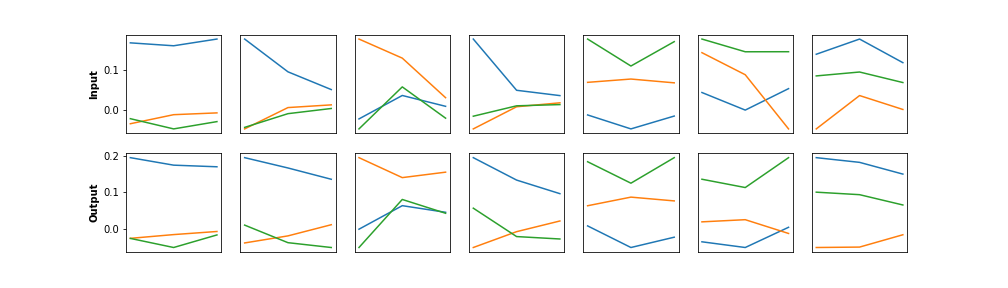
\includegraphics[width=\textwidth]{imagenes/Cap5/resultado_nn}
            \caption{Resultados de la red \textbf{NN\_33}}
            \label{fig:res_nn}
        \end{subfigure}       
        \begin{subfigure}[h]{0.99\textwidth} 
            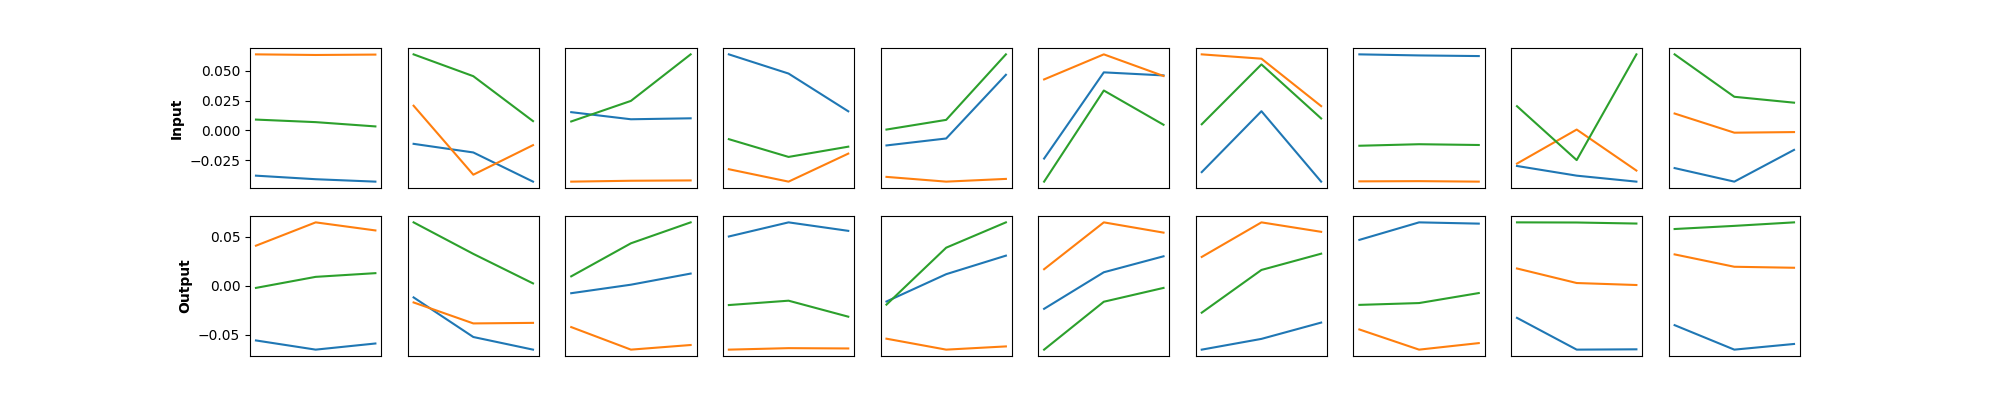
\includegraphics[width=\textwidth]{imagenes/Cap5/resultado_cnn}
            \caption{Resultados de la red \textbf{CNN\_33}}
            \label{fig:res_cnn}
        \end{subfigure}
        
        \begin{subfigure}[h]{0.99\textwidth} 
            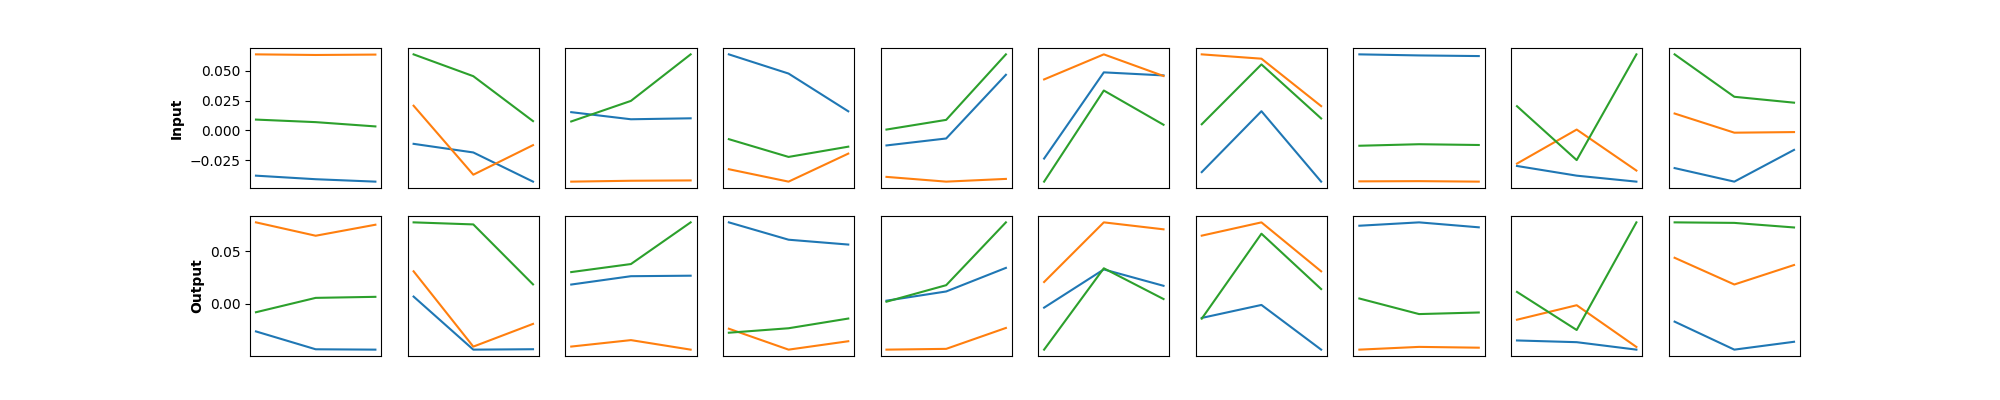
\includegraphics[width=\textwidth]{imagenes/Cap5/resultado_rnn}
            \caption{Resultados de la red \textbf{RNN\_33}}
            \label{fig:res_rnn}
        \end{subfigure}     
        \caption{Resultados.}
        
		\label{fig:res_autoencoders}
    \end{figure}


\vspace{5mm} %5mm vertical space
Como se puede observar las redes \textbf{NN\_33} y \textbf{CNN\_33} obtienen resultados m\'{a}s suavisados de las secuencias, debido a ello muchas veces la reconstrucci\'{o}n no se parece a la secuencia de entrada, por otra parte la red \textbf{RNN\_33} a pesar de tener un procesamiento m\'{a}s lento obtiene resultados mucho m\'{a}s similares a los de las entradas, lo cual es justo lo que se necesita en el presente trabajo. Por lo tanto, la red \textbf{RNN\_33} ser\'{a} el modelo ajustado al comportamiento normal de manejo.

\vspace{5mm} %5mm vertical space

Una vez definido como esta constituido el modelo del comportamiento normal de manejo se puede proceder con la elecci\'{o}n del m\'{e}todo de detecci\'{o}n de valores at\'{i}picos.

\subsection{M\'{e}todo de detecci\'{o}n de anomal\'{i}as}

Al inicio de esta secci\'{o}n se defini\'{o} tres diferentes enfoques para la detecci\'{o}n de anomal\'{i}as: la umbralizaci\'{o}n, la aplicaci\'{o}n de bosques de aislamiento y finalmente la aplicaci\'{o}n de SVM para una clase.

\vspace{5mm} %5mm vertical space

\subsubsection{Umbralizaci\'{o}n}

Para la aplicaci\'{o}n de umbralizaci\'{o}n se usar\'{a} la reconstrucci\'{o}n del error

, en cuanto para los bosques aleatorios y SVM de una clase se usar\'{a} el resultado del codificador de los autoencoders para su entrenamiento.


\section{Evaluaci\'{o}n del modelo de detecci\'{o}n de anomal\'{i}as}

